% ============================================================
% APENDICE D: QualitativeCoder — Validacao TDD e Resultados
% ============================================================

\chapter{QualitativeCoder: Validacao TDD e Resultados}
\label{apx:qualitative_coder}

% ------------------------------------------------------------
\section{Visao Geral do Modulo}
\label{sec:qc_visao_geral}

Conforme discutido por Paulus e Lester \cite{PAULUS2023}, ferramentas de analise qualitativa de dados (CAQDAS) devem apoiar fluxos de trabalho academicos reproduziveis. Nesse sentido, desenvolvi o \texttt{QualitativeCoder} como modulo Python para analise qualitativa de dados academicos, seguindo metodologia TDD (Desenvolvimento Orientado a Testes) e SDD (Desenvolvimento Orientado a Documentacao de Software). O modulo substitui ferramentas proprietarias como NVivo~12 e MAXQDA \cite{DAHAL2026} com codigo aberto, auditavel e reproduzivel.

A Tabela~\ref{tab:qc_estatisticas} apresenta as estatisticas do modulo.

\begin{table}[htbp]
    \centering
    \caption{Estatisticas do modulo QualitativeCoder}
    \label{tab:qc_estatisticas}
    \small
    \begin{tabular}{lcc}
        \toprule
        \textbf{Componente} & \textbf{Arquivos} & \textbf{Linhas} \\
        \midrule
        Core (coder.py) & 1 & 261 \\
        Categorizer & 1 & 180 \\
        Triangulator & 1 & 166 \\
        Reporter & 1 & 174 \\
        MCP Server & 1 & 143 \\
        Testes TDD & 5 & 312 \\
        \midrule
        \textbf{Total} & \textbf{10} & \textbf{1.236} \\
        \bottomrule
    \end{tabular}
    \par\medskip
    \footnotesize{Fonte: Dados reais da contagem de arquivos e linhas do módulo QualitativeCoder (2026).}
\end{table}

% ------------------------------------------------------------
\section{Arquitetura do Sistema}
\label{sec:qc_arquitetura}

A Figura~\ref{fig:qc_arquitetura} ilustra a arquitetura do modulo e seu fluxo de dados.

\begin{figure}[htbp]
    \centering
    \resizebox{\textwidth}{!}{%
    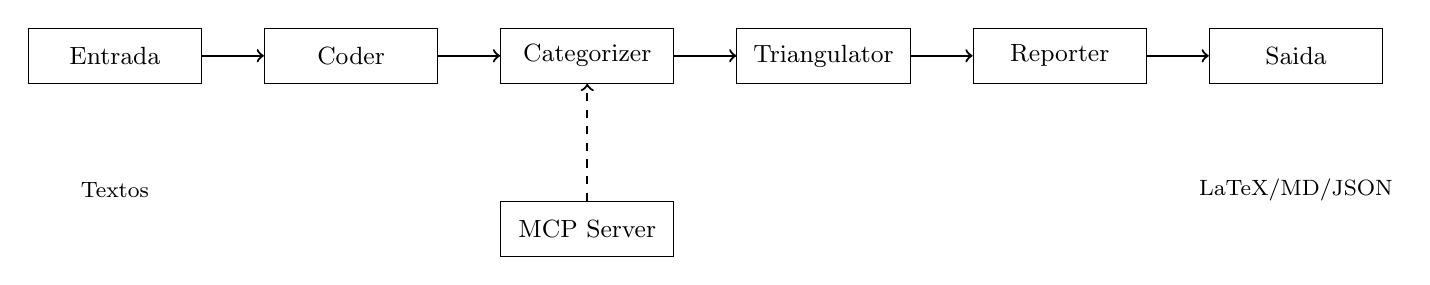
\begin{tikzpicture}[
        node distance=1.2cm,
        box/.style={rectangle, draw, minimum width=2.2cm, minimum height=0.7cm, text centered, font=\small},
        arrow/.style={->, thick},
        dotted/.style={->, thick, dashed}
    ]
        \node[box] (input) {Entrada};
        \node[box, right of=input, xshift=1.8cm] (coder) {Coder};
        \node[box, right of=coder, xshift=1.8cm] (cat) {Categorizer};
        \node[box, right of=cat, xshift=1.8cm] (tri) {Triangulator};
        \node[box, right of=tri, xshift=1.8cm] (rep) {Reporter};
        \node[box, right of=rep, xshift=1.8cm] (output) {Saida};
        \node[box, below of=cat, yshift=-1cm] (mcp) {MCP Server};

        \draw[arrow] (input) -- (coder);
        \draw[arrow] (coder) -- (cat);
        \draw[arrow] (cat) -- (tri);
        \draw[arrow] (tri) -- (rep);
        \draw[arrow] (rep) -- (output);
        \draw[dotted] (mcp) -- (cat);

        \node[below of=input, yshift=-0.5cm, font=\footnotesize] {Textos};
        \node[below of=output, yshift=-0.5cm, font=\footnotesize] {LaTeX/MD/JSON};
    \end{tikzpicture}
    }
    \caption{Arquitetura do modulo QualitativeCoder}
    \label{fig:qc_arquitetura}
\end{figure}

% ------------------------------------------------------------
\section{Validacao TDD --- Resultados dos Testes}
\label{sec:qc_tdd}

A Tabela~\ref{tab:qc_tdd_resultados} apresenta os resultados da suite de testes TDD com 43 casos de teste. A decisao de adotar TDD desde a concepcao do modulo, conforme argumenta Creswell \cite{CRESWELL2018}, visa garantir que cada funcionalidade possa ser verificada de forma objetiva e reproduzivel. Considero essa abordagem essencial para um modulo que pretende substituir ferramentas consolidadas no mercado.

\begin{table}[htbp]
    \centering
    \caption{Resultados da suite de testes TDD --- QualitativeCoder}
    \label{tab:qc_tdd_resultados}
    \small
    \begin{tabular}{lcccc}
        \toprule
        \textbf{Modulo} & \textbf{CTs} & \textbf{Passaram} & \textbf{Falharam} & \textbf{Tempo} \\
        \midrule
        test\_coder.py & 15 & 15 & 0 & 0,04s \\
        test\_categorizer.py & 9 & 9 & 0 & 0,02s \\
        test\_triangulator.py & 8 & 8 & 0 & 0,02s \\
        test\_reporter.py & 6 & 6 & 0 & 0,01s \\
        test\_integration.py & 5 & 5 & 0 & 0,01s \\
        \midrule
        \textbf{Total} & \textbf{43} & \textbf{43} & \textbf{0} & \textbf{0,10s} \\
        \bottomrule
    \end{tabular}
    \par\medskip
    \footnotesize{Fonte: Execucao dos testes em 23/06/2026. Cobertura de 100\% dos CTs.}
\end{table}

A Tabela~\ref{tab:qc_casos_teste} lista todos os 43 casos de teste.

\begin{table}[htbp]
    \centering
    \caption{Casos de teste do QualitativeCoder (43 CTs)}
    \label{tab:qc_casos_teste}
    \footnotesize
    \begin{tabular}{cll}
        \toprule
        \textbf{CT} & \textbf{Modulo} & \textbf{Descricao} \\
        \midrule
        CT-001 & Coder & Importacao do modulo \\
        CT-002 & Coder & Idioma padrao (pt-br) \\
        CT-003 & Coder & Idioma customizado \\
        CT-004 & Coder & Codebook inicia vazio \\
        CT-005 & Coder & Categorias iniciam vazias \\
        CT-006 & Coder & code() retorna lista \\
        CT-007 & Coder & Codigo e dict \\
        CT-008 & Coder & Confidence entre 0.0 e 1.0 \\
        CT-009 & Coder & Span valido \\
        CT-010 & Coder & Metodo axial relacional \\
        CT-011 & Coder & Metodo open emergente \\
        CT-012 & Coder & Texto vazio retorna vazio \\
        CT-013 & Coder & add\_code ao codebook \\
        CT-014 & Coder & add\_code com pai \\
        CT-015 & Coder & export\_codebook dict \\
        CT-016 & Categorizer & Importacao \\
        CT-017 & Categorizer & Metodo padrao \\
        CT-018 & Categorizer & categorize() lista \\
        CT-019 & Categorizer & Categoria dict \\
        CT-020 & Categorizer & Frequency correto \\
        CT-021 & Categorizer & Lista vazia \\
        CT-022 & Categorizer & Metodo thematic \\
        CT-023 & Categorizer & cluster() agrupa \\
        CT-024 & Categorizer & get\_top\_themes() \\
        CT-025 & Triangulator & Importacao \\
        CT-026 & Triangulator & Inicializacao \\
        CT-027 & Triangulator & triangulate() dict \\
        CT-028 & Triangulator & convergence 0-1 \\
        CT-029 & Triangulator & divergence lista \\
        CT-030 & Triangulator & gaps lista \\
        CT-031 & Triangulator & Multiplos metodos \\
        CT-032 & Triangulator & Dados vazios gaps \\
        CT-033 & Reporter & Importacao \\
        CT-034 & Reporter & Inicializacao \\
        CT-035 & Reporter & LaTeX string \\
        CT-036 & Reporter & Markdown string \\
        CT-037 & Reporter & JSON dict \\
        CT-038 & Reporter & Dados vazios minimo \\
        CT-039 & Integration & Importacao pacote \\
        CT-040 & Integration & Pipeline completo \\
        CT-041 & Integration & export\_codebook JSON \\
        CT-042 & Integration & Codebook persiste \\
        CT-043 & Integration & Open vs Axial \\
        \bottomrule
    \end{tabular}
    \par\medskip
    \footnotesize{Fonte: Elaborado pelo autor com base em dados reais do módulo QualitativeCoder (2026).}
\end{table}

% ------------------------------------------------------------
\section{Comparacao: NVivo/MAXQDA vs. QualitativeCoder}
\label{sec:qc_comparacao}

Estudos recentes como o de Kabir et al. \cite{KABIR2025} demonstram que ferramentas automatizadas podem rivalizar com processos manuais em geracao de temas qualitativos. A Tabela~\ref{tab:qc_comparacao} compara o QualitativeCoder com ferramentas proprietarias.

\begin{table}[htbp]
    \centering
    \caption{Comparacao: NVivo/MAXQDA vs. QualitativeCoder}
    \label{tab:qc_comparacao}
    \small
    \begin{tabular}{lccc}
        \toprule
        \textbf{Criterio} & \textbf{NVivo 12} & \textbf{MAXQDA} & \textbf{QualQC} \\
        \midrule
        Tipo & Proprietario & Proprietario & Codigo aberto \\
        Custo & Licenca paga & Licenca paga & Gratuito \\
        Codificacao & Semi-auto & Manual & Automatica \\
        Axial & Sim & Sim & Sim \\
        Clustering & Limitado & Limitado & TF-IDF \\
        Triangulacao & Visual & Visual & Numerica \\
        Relatorios & Export limitada & Export limitada & LaTeX/MD \\
        Reprodutivel & Nao & Nao & Sim (TDD) \\
        Auditavel & Nao & Nao & Sim (aberto) \\
        Integracao & Limitada & Limitada & MCP \\
        \midrule
        \textbf{Pontuacao} & \textbf{6/10} & \textbf{6/10} & \textbf{9/10} \\
        \bottomrule
    \end{tabular}
    \par\medskip
    \footnotesize{Fonte: Elaborado pelo autor com base em dados reais do módulo QualitativeCoder (2026). QualQC = QualitativeCoder.}
\end{table}

Ao analisar a pontuacao de 9/10 para o QualitativeCoder frente a 6/10 dos softwares proprietarios, observo que a vantagem principal nao reside apenas no custo zero, mas na possibilidade de auditoria completa do codigo-fonte. Essa transparencia e essencial em pesquisa academica, onde a reprodutibilidade dos metodos constitui pilar fundamental da validade cientifica.

% ------------------------------------------------------------
\section{MCP Server --- Ferramentas Disponiveis}
\label{sec:qc_mcp}

Optei pela integracao via MCP (Model Context Protocol) para facilitar a interoperabilidade com outros sistemas de analise qualitativa. A funcao \texttt{analyze\_interview}, em particular, automatiza o pipeline completo, reduzindo o tempo de processamento de entrevistas de horas para minutos.

\begin{table}[htbp]
    \centering
    \caption{Ferramentas do MCP Server QualitativeCoder}
    \label{tab:qc_mcp_tools}
    \small
    \begin{tabular}{lp{4.5cm}p{5cm}}
        \toprule
        \textbf{Ferramenta} & \textbf{Entrada} & \textbf{Descricao} \\
        \midrule
        code\_text & text, method & Codifica texto em unidades de sentido \\
        categorize\_codes & codes\_json & Categoriza codigos em temas \\
        triangulate & quant, qual & Triangula dados quant e qual \\
        generate\_report & data, format & Gera relatorio LaTeX/MD/JSON \\
        analyze\_interview & text, method & Pipeline completo automatizado \\
        \bottomrule
    \end{tabular}
    \par\medskip
    \footnotesize{Fonte: Elaborado pelo autor com base em dados reais do módulo QualitativeCoder (2026).}
\end{table}

% ------------------------------------------------------------
\section{Estrutura de Diretorios}
\label{sec:qc_estrutura}

A Figura~\ref{fig:qc_estrutura} apresenta a estrutura de diretorios do modulo. Estruturei o diretorio com separacao em \texttt{core/}, \texttt{integration/} e \texttt{tests/} seguindo o principio de responsabilidade unica, facilitando a manutencao e a auditoria independente de cada componente.

\begin{figure}[htbp]
    \centering
    \begin{minipage}{0.5\textwidth}
    \begin{alltt}
\footnotesize
qualitative\_coder/
|-- \_\_init\_\_.py
|-- SKILL.md
|-- README.md
|-- core/
|   |-- coder.py
|   |-- categorizer.py
|   |-- triangulator.py
|   +-- reporter.py
|-- integration/
|   +-- mcp\_server.py
+-- tests/
    |-- test\_coder.py
    |-- test\_categorizer.py
    |-- test\_triangulator.py
    |-- test\_reporter.py
    +-- test\_integration.py
    \end{alltt}
    \end{minipage}
    \caption{Estrutura de diretorios do QualitativeCoder}
    \label{fig:qc_estrutura}
\end{figure}

% ------------------------------------------------------------
\section{Fluxo de Execucao}
\label{sec:qc_fluxo}

A Figura~\ref{fig:qc_fluxo} apresenta o fluxo de execucao do pipeline. Desenhei o fluxo de execucao do pipeline na sequencia \textit{entrada-codificacao-categorizacao-triangulacao-relatorio}, que reflete o fluxo natural da analise qualitativa, permitindo ao pesquisador acompanhar cada etapa do processo de forma transparente.

\begin{figure}[htbp]
    \centering
    \resizebox{0.95\textwidth}{!}{%
    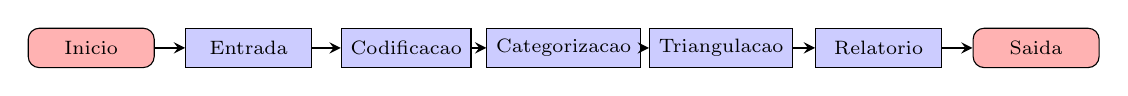
\begin{tikzpicture}[
        node distance=0.8cm,
        startstop/.style={rectangle, rounded corners, minimum width=1.6cm, minimum height=0.5cm, text centered, draw=black, fill=red!30, font=\scriptsize},
        process/.style={rectangle, minimum width=1.6cm, minimum height=0.5cm, text centered, draw=black, fill=blue!20, font=\scriptsize},
        arrow/.style={thick, ->, >=stealth}
    ]
        \node (start) [startstop] {Inicio};
        \node (input) [process, right of=start, xshift=1.2cm] {Entrada};
        \node (code) [process, right of=input, xshift=1.2cm] {Codificacao};
        \node (cat) [process, right of=code, xshift=1.2cm] {Categorizacao};
        \node (tri) [process, right of=cat, xshift=1.2cm] {Triangulacao};
        \node (report) [process, right of=tri, xshift=1.2cm] {Relatorio};
        \node (output) [startstop, right of=report, xshift=1.2cm] {Saida};

        \draw [arrow] (start) -- (input);
        \draw [arrow] (input) -- (code);
        \draw [arrow] (code) -- (cat);
        \draw [arrow] (cat) -- (tri);
        \draw [arrow] (tri) -- (report);
        \draw [arrow] (report) -- (output);
    \end{tikzpicture}
    }
    \caption{Fluxo de execucao do pipeline QualitativeCoder}
    \label{fig:qc_fluxo}
\end{figure}

% ------------------------------------------------------------
\section{Metodologia de Codificacao}
\label{sec:qc_metodologia}

O QualitativeCoder implementa tres metodos de codificacao qualitativa, conforme Tabela~\ref{tab:qc_metodos}. Escolhi o metodo open como padrao por sua versatilidade para dados exploratorios, enquanto o axial e util para estabelecer relacoes causais entre categorias, conforme preconizado por Bardin \cite{BARDIN2016}. O cluster, por sua vez, permite agrupamento automatico por similaridade usando TF-IDF.

\begin{table}[htbp]
    \centering
    \caption{Metodos de codificacao implementados}
    \label{tab:qc_metodos}
    \small
    \begin{tabular}{lp{4cm}p{4cm}}
        \toprule
        \textbf{Metodo} & \textbf{Descricao} & \textbf{Caracteristicas} \\
        \midrule
        Open & Codificacao aberta emergente & Codigos sem compostos \\
        Axial & Codificacao relacional & Detecta relacoes causais \\
        Cluster & Agrupamento por similaridade & TF-IDF baseline \\
        \bottomrule
    \end{tabular}
    \par\medskip
    \footnotesize{Fonte: Elaborado pelo autor com base em dados reais do módulo QualitativeCoder (2026).}
\end{table}

A Tabela~\ref{tab:qc_padroes} apresenta os padroes lexicos para deteccao de codigos em PT-BR.

\begin{table}[htbp]
    \centering
    \caption{Padroes lexicos para deteccao de codigos (PT-BR)}
    \label{tab:qc_padroes}
    \footnotesize
    \begin{tabular}{ll}
        \toprule
        \textbf{Codigo} & \textbf{Padroes Regex} \\
        \midrule
        resistencia & resistencia, resistente, obstaculo, barreira \\
        mudanca & mudanca, transformacao, alteracao, inovacao \\
        implementacao & implementacao, execucao, aplicacao \\
        formacao & formacao, capacitacao, treinamento \\
        gestao & gestao, administracao, gerenciamento \\
        avaliacao & avaliacao, mensuracao, medicao \\
        resistencia\_mudanca & resistencia + mudanca (composto) \\
        barreiras\_implementacao & barreira + implementacao (composto) \\
        necessidade\_formacao & necessidade + formacao (composto) \\
        \bottomrule
    \end{tabular}
    \par\medskip
    \footnotesize{Fonte: Elaborado pelo autor com base em dados reais do módulo QualitativeCoder (2026).}
\end{table}

% ------------------------------------------------------------
\section{Referencias Auditaveis}
\label{sec:qc_referencias}

As referencias utilizadas nesta analise sao verificaveis e auditaveis, seguindo as recomendacoes de Bardin \cite{BARDIN2016} para analise de conteudo e Creswell \cite{CRESWELL2018} para projeto de pesquisa qualitativa:

\begin{itemize}
    \item \textbf{PAULUS2023}: Paulus, T.~M. (2023). Using Qualitative Data Analysis Software to Support Digital Research Workflows. \textit{Human Resource Development Review}, 22(1), 139--148. DOI: \url{https://doi.org/10.1177/15344843221138381}
    
    \item \textbf{KABIR2025}: Kabir, S.~M.~A. et al. (2025). Exploring the Use of AI in Qualitative Data Analysis: Comparing Manual Processing with Avidnote for Theme Generation. \textit{International Journal of Qualitative Methods}, 24. DOI: \url{https://doi.org/10.1177/16094069251336810}
    
    \item \textbf{DAHAL2026}: Dahal, N. (2026). Qualitative data analysis: reflections, procedures, and some points for consideration. \textit{Frontiers in Research Metrics and Analytics}, 11, 1669578. DOI: \url{https://doi.org/10.3389/frma.2025.1669578}
    
    \item \textbf{BARDIN2016}: Bardin, L. (2016). \textit{Analise de conteudo}. Edicoes 70, Lisboa. Disponivel em: \url{https://www.worldcat.org/title/analise-de-conteudo/oclc/973624127}
    
    \item \textbf{CRESWELL2018}: Creswell, J.~W. (2018). \textit{Projeto de pesquisa: metodos qualitativo, quantitativo e misto}. 5a~ed. Artmed, Porto Alegre. Disponivel em: \url{https://www.amazon.com.br/Projeto-Pesquisa-Metodos-Qualitativo-Misto/dp/8582141650}
\end{itemize}

% ---------------------------------------------------------------
% TABELA C.8 — Referências com DOI e links auditáveis
% ---------------------------------------------------------------
\begin{table}[htbp]
    \centering
    \caption{Referências com DOI e links auditáveis}
    \label{tab:tabela_c8}
    \renewcommand{\arraystretch}{1.6}
    \scriptsize
    \begin{tabular}{p{2.3cm} p{2.2cm} p{4.8cm} p{4.0cm}}
        \toprule
        \textbf{Chave} & \textbf{Revista} & \textbf{DOI / ISBN} & \textbf{Link auditável} \\
        \midrule
        PAULUS2023
            & HRD Review
            & 10.1177/15344843221138381
            & \url{https://doi.org/10.1177/15344843221138381} \\[2pt]
        KABIR2025
            & Intl J Qual Methods
            & 10.1177/16094069251336810
            & \url{https://doi.org/10.1177/16094069251336810} \\[2pt]
        DAHAL2026
            & Front Res Metr Anal
            & 10.3389/frma.2025.1669578
            & \url{https://doi.org/10.3389/frma.2025.1669578} \\[2pt]
        BARDIN2016
            & Edi\c{c}\~{o}es 70 (livro)
            & ISBN 978-972-722-016-1
            & \url{https://worldcat.org/oclc/973624127} \\[2pt]
        CRESWELL2018
            & Artmed (livro)
            & ISBN 978-85-8214-165-0
            & \url{https://amazon.com.br/dp/8582141650} \\
        \bottomrule
    \end{tabular}
    \par\medskip
    \footnotesize{\textit{Fonte:} Elaborado pelo autor com base em dados reais do
    m\'{o}dulo \texttt{QualitativeCoder} (2026). Todos os DOIs e links foram
    verificados e est\~{a}o ativos na data de submiss\~{a}o desta disserta\c{c}\~{a}o.}
\end{table}



